% ============================================================
% Research Proposal (v2, restructured) - Bar Mordechai Damri
% Ben-Gurion University of the Negev
% Supervisors: Prof. Roni Stern, Prof. Rami Puzis
% Compile: xelatex research_proposal_v2.tex -> bibtex research_proposal_v2 -> xelatex x2
% ============================================================

\documentclass[12pt,a4paper]{article}

\usepackage{fontspec}
\usepackage{polyglossia}
\setmainlanguage{english}
\setotherlanguage{hebrew}
\newfontfamily\hebrewfont[Script=Hebrew,BoldFont=Arial Hebrew Bold]{Arial Hebrew}

\usepackage{geometry}
\geometry{a4paper, left=2.5cm, right=2.5cm, top=2.3cm, bottom=2.5cm}

\usepackage{microtype}
\usepackage{setspace}
\setstretch{1.5}

\usepackage{xcolor}
\definecolor{bgunavy}{RGB}{27,61,110}
\usepackage{titlesec}
\titleformat{\section}{\large\bfseries\color{bgunavy}}{\thesection.}{0.6em}{}
\titleformat{\subsection}{\normalsize\bfseries\color{bgunavy}}{\thesubsection}{0.5em}{}
\titleformat{\subsubsection}{\normalsize\bfseries\itshape}{\thesubsubsection}{0.5em}{}
\titlespacing*{\section}{0pt}{10pt}{3pt}
\titlespacing*{\subsection}{0pt}{7pt}{2pt}
\titlespacing*{\subsubsection}{0pt}{5pt}{1pt}

\usepackage{amsmath}
\usepackage{amssymb}
\usepackage{booktabs}
\usepackage{tabularx}
\usepackage{array}
\usepackage{enumitem}
\setlist[itemize]{topsep=2pt,itemsep=1pt,parsep=0pt,leftmargin=1.3em}
\setlist[enumerate]{topsep=2pt,itemsep=1pt,parsep=0pt,leftmargin=1.6em}

\usepackage{hyperref}
\hypersetup{colorlinks=true, linkcolor=bgunavy, citecolor=bgunavy, urlcolor=bgunavy,
  pdftitle={Research Proposal - Bar Mordechai Damri}, pdfauthor={Bar Mordechai Damri}}

\setlength{\parindent}{0pt}
\setlength{\parskip}{4pt}

\usepackage{float}
\usepackage{caption}
\usepackage{subcaption}
\captionsetup{font=small, labelfont=bf, skip=3pt}
\usepackage{multicol}
\setlength{\columnsep}{18pt}
\usepackage{graphicx}
\graphicspath{{figures/}}
\usepackage{colortbl}
\usepackage{algorithm}
\usepackage{algpseudocode}
\usepackage[round]{natbib}
\setlength{\bibsep}{2pt}

\newcommand{\dist}{d}
\newcommand{\simf}{\mathrm{sim}}

\begin{document}

% ============================================================
% COVER PAGE
% ============================================================
\begin{titlepage}
\centering\singlespacing
\vspace*{0.1cm}

\includegraphics[height=2.1cm]{bgu_logo.png}\\[10pt]
{\large\bfseries Ben-Gurion University of the Negev}\\[5pt]
{\normalsize The Stein Faculty of Computer and Information Science}\\[3pt]
{\normalsize The Institute for the Foundations of Artificial Intelligence}

\vspace{2.2cm}
{\LARGE\bfseries\color{bgunavy}\setstretch{1.2}
Embedding Geometric Heuristics for\\
Improving RAG Systems
}

\vspace{0.8cm}
\begin{otherlanguage*}{hebrew}
{\Large\bfseries
הטמעת יוריסטיקות גיאומטריות לשיפור מערכות \textenglish{\LR{RAG}}
}
\end{otherlanguage*}

\vspace{1.8cm}
{\large\itshape Research proposal}

\vspace{1.8cm}
{\large\bfseries Bar Mordechai Damri \,\texthebrew{בר מרדכי דמרי}}\\[6pt]
{\normalsize Student ID: 208915751}

\vspace{1.6cm}
{\normalsize Supervisors:}\\[8pt]
{\large\bfseries Prof. Roni Stern \quad Prof. Rami Puzis}

\vfill
\end{titlepage}

% ============================================================
% ABSTRACT
% ============================================================
\setcounter{page}{2}
\section*{Abstract}

Retrieval-Augmented Generation (RAG) is the standard way to let a large language model answer questions about documents it was never trained on. A component called the retriever first finds a few documents that seem relevant to the question, and the language model then writes an answer based on them. If the retriever brings the wrong documents, the answer is wrong, no matter how good the language model is. Today's retrievers turn every question and every document into a point in a high-dimensional space and return the documents whose points are closest to the question's point. This works only if a question really does land close to the documents that answer it. That assumption is rarely examined, and this research examines it directly.

The research has three goals. The first is to study the geometric properties of the space in which a retriever places questions and documents: where a question lands relative to the documents that answer it, and what distinguishes the questions on which the retriever succeeds from those on which it fails. The second is to develop simple geometric heuristics, built on what the first goal discovers, that improve retrieval by moving the starting point of the search away from the question and toward the region where the relevant documents are. The third is to develop iterative search algorithms for the cases in which the retriever fails: algorithms that inspect documents one at a time and keep moving the starting point as evidence accumulates. The three goals are evaluated on a benchmark collection of biomedical questions in which every question-document pair has already been scored for relevance, so that any method can be compared against the standard retriever offline, and the results are validated on two public collections from other domains.

\begin{otherlanguage*}{hebrew}\sloppy\setlength{\emergencystretch}{3em}
\subsection*{\texthebrew{תקציר}}
\textenglish{\LR{RAG}} היא הדרך המקובלת לאפשר למודל שפה גדול לענות על שאלות לגבי מסמכים שהוא מעולם לא אומן עליהם. רכיב שנקרא מנגנון השליפה מוצא תחילה כמה מסמכים שנראים רלוונטיים לשאלה, ומודל השפה כותב תשובה על בסיסם. אם השליפה מביאה את המסמכים הלא נכונים, התשובה שגויה, לא משנה כמה טוב מודל השפה. מנגנוני השליפה של היום הופכים כל שאלה וכל מסמך לנקודה במרחב רב-ממדי, ומחזירים את המסמכים שהנקודות שלהם הקרובות ביותר לנקודה של השאלה. זה עובד רק אם השאלה אכן נוחתת קרוב למסמכים שעונים עליה. ההנחה הזו כמעט לא נבדקת, והמחקר הזה בודק אותה ישירות.

למחקר שלוש מטרות. הראשונה היא לחקור את התכונות הגיאומטריות של המרחב שבו מנגנון השליפה ממקם שאלות ומסמכים: היכן שאלה נוחתת ביחס למסמכים שעונים עליה, ומה מבדיל בין השאלות שבהן השליפה מצליחה לאלה שבהן היא נכשלת. השנייה היא לפתח יוריסטיקות גיאומטריות פשוטות, שנשענות על מה שהמטרה הראשונה מגלה, שמשפרות את השליפה על ידי הזזת נקודת ההתחלה של החיפוש מהשאלה לכיוון האזור שבו נמצאים המסמכים הרלוונטיים. השלישית היא לפתח אלגוריתמי חיפוש איטרטיביים למקרים שבהם השליפה נכשלת: אלגוריתמים שבודקים מסמך אחר מסמך וממשיכים להזיז את נקודת ההתחלה ככל שמצטברות ראיות. שלוש המטרות מוערכות על אוסף מבחן של שאלות ביו-רפואיות שבו כל זוג שאלה-מסמך כבר קיבל ציון רלוונטיות, כך שכל שיטה ניתנת להשוואה מול השליפה הסטנדרטית באופן לא מקוון, והתוצאות מאומתות על שני אוספים ציבוריים מתחומים אחרים.
\end{otherlanguage*}

% ============================================================
% GLOSSARY
% ============================================================
\enlargethispage{3\baselineskip}
\section*{Terms used in this proposal}

\noindent\begin{minipage}{\textwidth}
\footnotesize\setstretch{1.0}\renewcommand{\arraystretch}{1.18}
\begin{tabularx}{\textwidth}{>{\raggedright\arraybackslash}p{3.7cm}>{\raggedright\arraybackslash}X}
\toprule
Term & Meaning in this proposal \\
\midrule
Large language model (LLM) & A neural network trained on very large amounts of text that can read a prompt and write fluent text in response (for example, GPT or Gemini). \\
Embedding & A list of numbers (a vector) that a neural network produces to represent a piece of text. Texts with similar meaning get similar vectors. \\
Embedding space & The high-dimensional space in which these vectors live. Each question and document is one point in it (768 dimensions in this work). \\
Normalized vector & A vector scaled so that its length is exactly 1. All embeddings in this work are normalized, so that only their direction matters; cosine similarity then reduces to a plain dot product, which is also cheaper to compute. \\
Cosine similarity / distance & The standard way to compare two embeddings: the cosine of the angle between the two vectors (1 = same direction, 0 = unrelated). Distance is $1 - \text{similarity}$, so smaller means closer. \\
Retriever & The component that returns, for a question, the documents it finds most relevant. \\
Bi-encoder & The common retriever design: one network turns the question into an embedding, one turns each document into an embedding, and the two are compared only afterwards. \\
Nearest-neighbor search & Returning the documents whose embeddings are closest to a given point. The \emph{pool} is the set of documents searched. \\
Search anchor & The point from which nearest-neighbor search is run. In a standard retriever it is the question's embedding; the central idea of this proposal is to move it. \\
Rank, Top-$k$ & The position of a document in a method's output list (1 = returned first); the top-$k$ are the $k$ documents ranked highest. \\
Ground truth (GT) & The one document the benchmark marks as the correct answer to a question. \\
Relevance judgment & A score saying how relevant a document is to a question. Here the scores come from an LLM acting as a judge, on a scale from 0.1 (irrelevant) to 1.0 (fully relevant). \\
Centroid & The average of a set of embeddings, scaled back to length 1: the ``center of mass'' of a group of documents. \\
Oracle & A quantity that uses information a real system would not have at run time (for example, a centroid built from all relevance judgments); used to measure what is possible. \\
Inspection budget & How many documents a method may send to the judge before it must stop. \\
Benchmark & A fixed set of questions, documents and answers on which methods are compared fairly. \\
\bottomrule
\end{tabularx}
\end{minipage}


% ============================================================
% 1. BACKGROUND
% ============================================================
\section{Scientific background}

This section builds up the problem in four steps. It first explains what a RAG system is and why its retriever decides the quality of the final answer. It then describes how retrievers are built today and introduces the idea of a \emph{search anchor}, which is the object this research works on. It then explains why retrievers are not perfect, using what is known about the geometry of embedding spaces. Finally it presents our approach and what has been done so far.

\subsection{What is RAG}

A large language model (LLM) answers questions from what it absorbed during training. That knowledge is frozen on the day training ends and does not include private or specialized documents. Retrieval-Augmented Generation (RAG) fixes this by adding a search step in front of the model \citep{lewis2020rag}. A RAG system has three components:
\begin{enumerate}
  \item An \textbf{indexer}, which runs once in advance: it turns every document in a collection into an embedding (a vector of numbers that captures the document's meaning) and stores all the vectors.
  \item A \textbf{retriever}, which runs for every question: it turns the question into an embedding in the same way, finds the documents whose embeddings are closest to it, and returns the top few.
  \item A \textbf{generator}, the LLM itself: it receives the question together with the retrieved documents and writes the answer from them.
\end{enumerate}

Many variations of this pipeline exist. Some feed many retrieved passages to the generator at once \citep{izacard2021fid}, some let the model decide when it needs to retrieve \citep{jiang2023flare,asai2024selfrag}, and a recent survey organizes the whole family \citep{gao2023ragsurvey}. What all variations share is the dependence on the retriever: if the document that holds the answer is not among the retrieved ones, the generator cannot produce a correct grounded answer, and documents that are irrelevant actively push it toward wrong answers \citep{shi2023distractors}. The quality of the retriever is therefore an upper bound on the quality of the whole system, and it is the retriever that this research studies.

\textbf{How the retriever decides what is close.} The standard retriever is a \emph{bi-encoder} \citep{karpukhin2020dpr}: the same kind of neural network encodes questions and documents separately into vectors of the same length (768 numbers in our case). Each vector is scaled to length 1, so that only its direction carries meaning, and the retriever ranks documents by the \emph{cosine similarity} between the question's vector and each document's vector. Cosine similarity is the cosine of the angle between two vectors: 1 when they point in the same direction, 0 when they are unrelated. Returning the documents with the highest similarity is called \emph{nearest-neighbor search}. The whole design rests on one assumption: that a question's vector lands close to the vectors of the documents that answer it.

\subsection{How retrievers are implemented today}

\textbf{Overview of approaches.} Research on retrievers has improved every part of the design except that assumption. One line trains better encoders, so that similar meanings map to closer vectors: the network is trained to pull matching question-document pairs together and push other pairs apart, on unlabeled text \citep{izacard2022contriever}, on web-scale weak labels \citep{wang2022e5}, with instructions attached to the text \citep{su2023instructor}, and with carefully chosen ``hard negatives'', documents that are close to the question but wrong \citep{qu2021rocketqa,xiong2021ance}. A second line scores documents in a richer way than one cosine between two vectors: one vector per word \citep{khattab2020colbert}, or vectors with one entry per vocabulary word \citep{formal2021splade}. A third line adds a \emph{re-ranker}: a slower, stronger model, often an LLM, that re-orders the top candidates the retriever returned \citep{nogueira2020monot5,sun2023rankgpt}. A fourth line rewrites the question before encoding it, for example by asking an LLM to write a short hypothetical answer and searching with that text instead; the best-known version is called HyDE \citep{wang2023query2doc,gao2023hyde}. A fifth line, the oldest, is \emph{relevance feedback}: take the top-ranked documents (the top-$k$), assume they are relevant, and move the question's vector toward their average; this is known as the Rocchio update \citep{rocchio1971relevance}, and it works on embeddings as well as on words \citep{li2023vectorprf}. A recent survey covers all of these \citep{zhao2024densesurvey}.

\textbf{What is a search anchor.} In every method above, the search is run from some point in the embedding space, and the documents returned are the nearest neighbors of that point. We call that point the \emph{search anchor}. In a standard retriever, the anchor is the question's embedding. Rewriting methods replace it by the embedding of the rewritten text. Relevance feedback moves it toward the top-ranked documents. A few recent methods move it using feedback from an LLM: TOUR adjusts the anchor step by step, using a re-ranker's opinions as a stand-in for relevance labels \citep{sung2023tour}; ReDE-RF asks an LLM which first-pass documents are relevant and searches from their embeddings instead \citep{jataria2024rederf}; BAGEL spends a limited number of LLM judgments to explore the space \citep{bagel2026}. Re-rankers, by contrast, never move the anchor: they only re-order what the anchor already found. The distinction matters, because a document that the anchor misses stays missed no matter how good the re-ranker is.

\subsection{Gap: why retrievers are not perfect}

Even the best retrievers rank the correct document first for only part of the questions, and the failures are not random. Two kinds of knowledge about the embedding space help explain why.

\textbf{What is known about the space.} The vectors a neural network produces do not spread out evenly in all directions. They crowd into a narrow cone, so that even two unrelated texts have a fairly high cosine similarity, and the differences that matter are squeezed into a small range \citep{ethayarajh2019contextual}. In spaces with many dimensions, some points also become ``hubs'': they are among the nearest neighbors of a great many other points, for no semantic reason \citep{radovanovic2010hubs}. And a single vector per text can only separate so many documents from one another \citep{luan2021sparse}. The usual remedies apply the same correction to every vector, for example removing the directions that all vectors share \citep{mu2018allbutthetop}; such corrections also help retrievers \citep{jung2023isotropic}. There is also evidence that questions and documents are not placed in the space in the same way: a bi-encoder never sees a question and a document together, the training objective pulls questions toward documents but not the reverse \citep{li2021dance}, and the choice of sharing or separating the two encoders changes where the two populations land \citep{dong2022dualencoder}.

\textbf{What is not known.} All of this describes the space as a whole. What has not been measured, to our knowledge, is the situation of one question at a time: where the question's point sits relative to the documents that are relevant to it, and relative to the one document marked as the correct answer. If a question systematically lands \emph{away} from its relevant documents, then nearest-neighbor search from the question's point is searching in the wrong place, and no re-ranker can fix that.

\textbf{How relevance is measured.} Studying this requires knowing, for many question-document pairs, how relevant the document is. Human labels do not exist at that scale, so we use an LLM as a \emph{judge}: it reads a question and a document and returns a score between 0.1 and 1.0. LLM judges agree with human assessors about as well as assessors agree with each other \citep{thomas2024llmjudge,upadhyay2024umbrela}, although they have known biases and should not be treated as the final word \citep{soboroff2024cantreplace}. In this proposal the judge is a measuring instrument: it tells us where the relevant documents are, so that the geometry can be measured. Its scores also reveal something that a single ``correct answer'' label hides: most questions have several documents that answer them equally well. We therefore count success in two ways throughout, reaching the labeled answer (\emph{exact success}) and reaching any document the judge rates as fully relevant (\emph{soft success}).

\subsection{Our approach}
\label{sec:approach}

Our approach is to measure first and design second. The first goal is to study the geometry of the retriever's space one question at a time: how dense the question's neighborhood is, how far it is from the documents that answer it, and which of these properties separate the questions the retriever solves from those it fails. The intention is a picture of the space that is precise enough to act on, and, as its practical output, a model that predicts from geometry alone whether the retriever will fail on a given question. The second goal takes what the first discovers and turns it into geometric heuristics: simple rules that move the search anchor from the question toward the region where the relevant documents lie, by an amount set from the measured geometry rather than fixed in advance. The intention is a better starting point for the search that any bi-encoder can use without retraining. The third goal addresses the cases where the retriever fails even so: iterative search algorithms that inspect documents one at a time, ask the judge about each, and move the anchor again after each answer, so that the search follows the evidence it collects. The intention is to reach a relevant document with as few inspections as possible exactly where the standard retriever needs the most help.

Each goal already has a first result behind it. For the first, we measured the space on a benchmark of 196 biomedical questions with a 5,035-document pool in which every pair is judged. The question's neighborhood holds 3 documents on average while the center of the relevant documents is surrounded by 10, the question is 44\% farther from the correct answer than that center is, and the questions on which the retriever fails differ from the others in these measurements. For the second, we compared the standard retriever with several fixed ways of blending the question with that center: a small pull toward it gains one point of accuracy, replacing the question by it loses most of the accuracy, and 79\% of the retriever's ``failures'' return a document the judge rates as fully relevant. For the third, a first prototype that moved the anchor by a fixed amount after every relevant hit made results worse, from 3.3 to 4.6 inspected documents on average; the analysis of why gives the design of the proposed algorithm.

% ============================================================
% 2. OBJECTIVES
% ============================================================
\section{Research objectives and expected significance}

The three goals correspond to three research questions.

\begin{enumerate}[label=\textbf{RQ\arabic*.}, leftmargin=2.6em]
  \item \textbf{What does the retriever's embedding space look like around a question, and does that geometry tell us when the retriever will fail?} Concretely: where does a question's point sit relative to its relevant documents and its correct answer, which measurable properties of the neighborhood separate solved questions from failed ones, and can a model built from those properties alone predict failure before any document is inspected?\\[2pt] \textit{Expected contribution:} a measured description of the space and a failure predictor that needs no relevance labels at run time.
  \item \textbf{Can a geometric heuristic that moves the search anchor improve retrieval?} If the anchor is moved from the question toward the relevant region, by an amount chosen from the geometry measured for RQ1, does the retriever find the correct document, or a fully relevant one, after inspecting fewer documents than the standard retriever?\\[2pt] \textit{Expected contribution:} a one-shot anchor heuristic and the conditions under which it helps.
  \item \textbf{For the questions on which the retriever fails, does an iterative search that keeps moving the anchor do better?} If the anchor is updated after every inspected document, using the judge's answer, does the search reach a relevant document faster than the one-shot heuristic and than existing feedback methods, at the same inspection budget?\\[2pt] \textit{Expected contribution:} an iterative algorithm, its cost-accuracy curve, and a comparison with the closest published methods.
\end{enumerate}

\textbf{Significance.} Retrieval quality bounds every RAG answer, yet the standard retriever rests on an assumption, that a question lands near its answers, that is not checked. Answering RQ1 gives a way to know in advance when that assumption fails for a given question. Answering RQ2 and RQ3 gives a way to act on it without retraining the encoder or re-indexing the collection: the heuristics operate on the vectors any bi-encoder already produces, so they can be added to an existing system. The biomedical benchmark is the place where the methods are compared, chosen because the gap between questions and documents is known to be large there; the findings are then validated on two public collections from other domains, so that the conclusions are about retrievers in general and not about one dataset.

% ============================================================
% 3. PROPOSED RESEARCH
% ============================================================
\section{Detailed description of the proposed research}

The research is organized in four phases. Phase~1 is the shared foundation: the benchmark on which everything is measured, the baselines against which everything is compared, and the measurements that motivate the rest; most of it is complete. Phases 2, 3 and 4 correspond to RQ1, RQ2 and RQ3. Each is described in the same way: what problem it solves, stated precisely; how we propose to solve it; and how the solution will be evaluated.

\textbf{Notation.} Before the phases, a few symbols that all of them share. A question is represented by its embedding, which we write $Q$; a document by its embedding, $d$; and the document the benchmark marks as the correct answer by $GT$. All embeddings are normalized to length 1, so the cosine similarity between two of them, written $\simf(x,y)$, is simply their dot product, and the cosine distance $\dist(x,y)=1-\simf(x,y)$ is 0 for identical vectors and grows as they point in different directions. The pool of documents is $\mathcal{D}$. The judge's relevance score for a document is $J(d)$, a number between 0.1 and 1.0. The set of documents the judge scores 1.0, the fully relevant ones, is $R$, and $C$ is the centroid of $R$: the average of their vectors, scaled back to length 1. Because $C$ uses the judge's score for every document in the pool, no running system could compute it; it is an oracle that tells us where the relevant region is, and we use it to measure what is possible. Later, when a method builds a centroid from only the documents it has inspected so far, we write that centroid with a subscript, $C_k$ or $C_t$, to make clear that it is not the oracle.

\subsection{Phase 1. Setup and benchmark}
\label{sec:phase1}

\textbf{The benchmark.} Comparing retrieval methods requires a fixed set of questions, a fixed set of documents, and, for each question, a way to tell how good every method's output is. The collection we use for this is a biomedical question-answering benchmark derived from PubMed, the main bibliographic database of the life sciences: 196 questions, each with one abstract marked as its correct answer, and a shared pool of 5,035 abstracts. We chose a biomedical collection as the benchmark, rather than a general one, because this is where the gap between questions and documents is known to be largest: retrievers trained on general text lose the most on biomedical tasks \citep{thakur2021beir}, the questions are short expert queries while the documents are dense scientific abstracts \citep{tsatsaronis2015bioasq}, and pre-training on biomedical text alone does not close the gap \citep{lee2020biobert,jin2023medcpt}. A large gap makes the geometry easier to measure and a method's improvement easier to see. The benchmark is where the methods are compared; the domain itself is not the object of the research, and Phases 2-4 each end with a validation on collections from other domains.

Every question and every document in the benchmark was embedded with the same publicly available bi-encoder (\texttt{all-mpnet-base-v2}, 768 dimensions). Then every question-document pair, about one million pairs, was scored for relevance by a Gemini-2.5-flash-lite judge; the scores fall almost entirely on six values (0.1, 0.2, 0.4, 0.6, 0.8, 1.0). This exhaustive judging is what makes the rest of the research practical. A retrieval method is, in the end, a rule for the order in which documents are inspected, and since the benchmark already holds the judge's answer for every document, any method can be simulated offline, on all 196 questions, in seconds, with no new LLM calls. The judging also showed that the correct answer is rarely unique: on average 17 documents per question receive the top score.

\textbf{Baseline retrievers.} A new method is only as convincing as the methods it is compared against, so Phase~1 fixes a set of baselines that spans the design space of Section~1.2 and can all be simulated on the benchmark. The first and most important is \textbf{B1}, the standard retriever, which ranks the pool by distance to the question, $\dist(d,Q)$; every other method must beat it. The second, \textbf{B2}, ranks the pool by distance to the oracle centroid, $\dist(d,C)$; it is not a deployable method, but it shows what searching from the center of the relevant region would give if that center were known. Between these two we placed three fixed blends, \textbf{H1-H3}: a weighted sum of the two distances, $\alpha\,\dist(d,Q)+(1-\alpha)\,\dist(d,C)$ for several values of $\alpha$; the question's order with the centroid breaking ties; and B1's top-$k$ re-ordered by distance to the centroid. These map out what a rule fixed in advance can do, and they are the reference point for the geometry-guided rules of Phases 3 and 4. Two baselines represent the feedback family: classic \textbf{relevance feedback}, in which B1's top-$k$ are judged and the anchor is moved to the centroid of those judged relevant \citep{li2023vectorprf}, and \textbf{LLM re-ranking}, in which B1's top-$k$ are re-ordered by the judge's score \citep{sun2023rankgpt}. All of these are implemented. The remaining baselines are the published anchor-moving methods, ReDE-RF \citep{jataria2024rederf} and TOUR \citep{sung2023tour}, and the hypothetical-document anchor of HyDE \citep{gao2023hyde}; implementing them on the benchmark is the open item of Phase~1.

\textbf{What the benchmark shows.} Table~\ref{tab:results} gives the main numbers and Figure~\ref{fig:trilateration} shows the geometry of two questions. Three results drive the rest of the proposal.

\begin{table}[H]
\centering\small
\caption{Where the correct document ends up in each method's output, over 196 questions. ``Mean rank'' is the average position of the correct document; ``Top-1'' is the share of questions where it is returned first.}
\label{tab:results}
\setstretch{1.05}
\begin{tabularx}{\textwidth}{>{\raggedright\arraybackslash}X*{4}{>{\centering\arraybackslash}p{1.5cm}}}
\toprule
Method & Mean rank & Top-1 (\%) & Top-3 (\%) & Top-10 (\%) \\
\midrule
B1: distance to the question (standard retriever) & 3.29 & 70.4 & 83.2 & 91.8 \\
B2: distance to the oracle centroid & 9.87 & 14.8 & 36.2 & 62.8 \\
H1: $0.93\,\dist(d,Q) + 0.07\,\dist(d,C)$                & 3.35 & 71.4 & 82.7 & 90.8 \\
H2: B1 order, centroid breaks ties & 3.29 & 70.4 & 83.2 & 91.8 \\
H3: B1's top-10 re-ordered by centroid & 5.05 & 17.9 & 43.9 & 91.8 \\
Relevance feedback (top-5, threshold 1.0) & 4.90 & 31.1 & -    & -    \\
LLM re-ranking of B1's top-5                             & 2.35 & 40.8 & -    & -    \\
\bottomrule
\end{tabularx}
\end{table}

\begin{figure}[H]
\centering
\begin{subfigure}[t]{0.49\textwidth}
  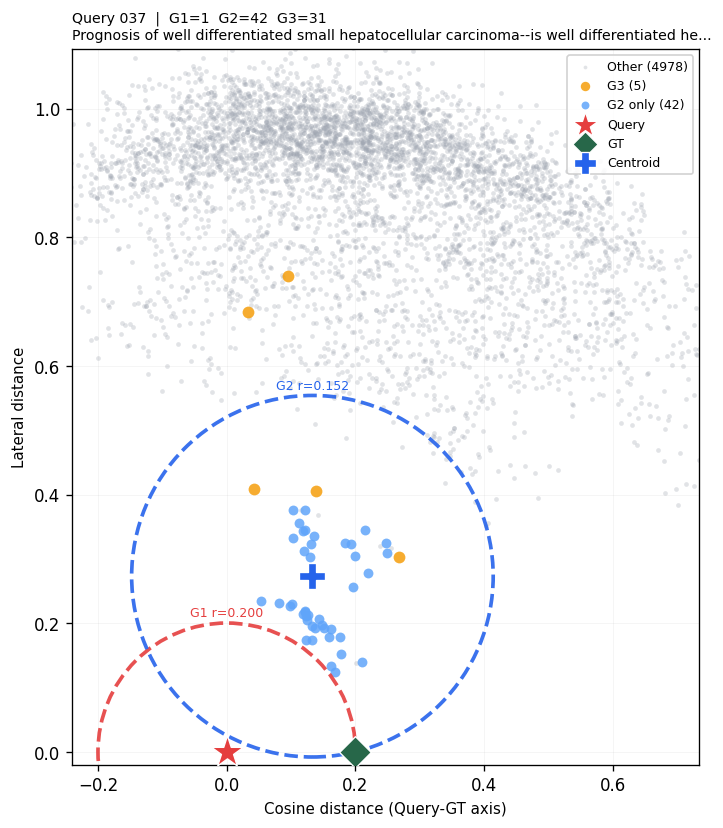
\includegraphics[width=\textwidth]{trilateration_q037.png}
  \caption{Question 37. One document lies within the question's circle; 42 lie within the centroid's circle.}
\end{subfigure}\hfill
\begin{subfigure}[t]{0.49\textwidth}
  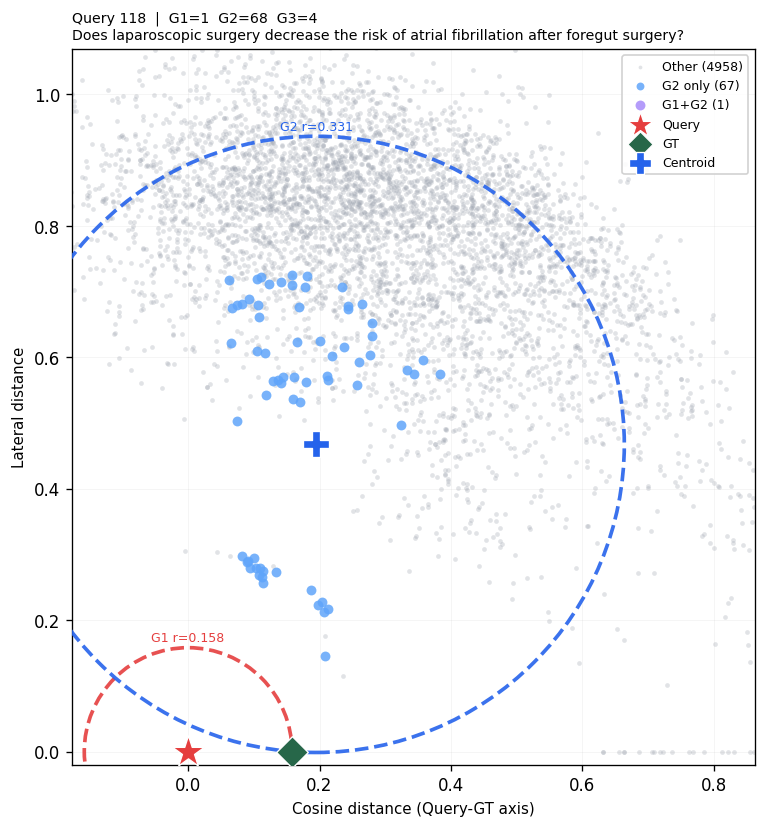
\includegraphics[width=\textwidth]{trilateration_q118.png}
  \caption{Question 118. Here the centroid is farther from the correct answer than the question is, yet its neighborhood is still dense.}
\end{subfigure}
\caption{The geometry of two questions, drawn so that distances to the question (red star) and to the correct answer (green diamond) are exact. The red circle around the question has radius $\dist(Q,GT)$: anything inside it is returned before the correct answer by the standard retriever. The blue circle is the same construction around the centroid $C$ (blue cross). Orange points are documents the judge scored 1.0.}
\label{fig:trilateration}
\end{figure}

\textbf{Result 1: questions are outliers.} For each question we draw a circle around it whose radius is its distance to the correct answer; every document inside that circle is returned before the correct answer. The circle holds 3.1 documents on average (median 1). The same circle drawn around the centroid $C$ holds 9.7 (median 6), while random points at the same distance from the correct answer hold 0.8, so the density around $C$ is real and not an artifact of the radius. The mean distances are $\dist(Q,GT)\approx\dist(Q,C)\approx0.17$ and $\dist(C,GT)\approx0.10$: the centroid is 44\% closer to the correct answer than the question is. The correct answer is not on the straight line between $Q$ and $C$ either; its mean perpendicular offset from that line is 0.39. The implication is that neither the question nor the centroid is, by itself, the right place to search from.

\textbf{Result 2: relevance is graded by distance.} Documents the judge scores 0.1 lie at mean distance 0.89 from the correct answer, and the distance falls step by step with the score: 0.84, 0.77, 0.63, 0.40, and 0.22 for score 1.0. The relation holds within every one of the 196 questions. The implication is twofold. The judge is a reliable instrument: when it says ``fully relevant'', the document is geometrically near the answer. But the judge cannot replace geometry: re-ordering B1's top-5 purely by the judge's score lowers Top-1 from 70.4\% to 40.8\%, because many documents share the top score and the labeled answer is only one of them.

\textbf{Result 3: fixed rules barely help, and most failures are soft.} In Table~\ref{tab:results}, a small fixed pull toward the centroid (H1) gains one point of Top-1 over B1; stronger pulls, tie-breaking, and re-ordering a window all lose, and replacing the question by a feedback centroid loses badly (31.1\%). Among the 58 questions where B1 does not rank the correct answer first, in 46 (79\%) the document it returns first is itself scored 1.0 by the judge, and every one of the 58 has a fully relevant document in its top 10. The implication is that a rule fixed in advance is not enough, and that exact and soft success must be reported side by side, as they are throughout this proposal.

\subsection{Phase 2. Characterizing the geometry and predicting retriever failure}

\textbf{Problem definition.} Phase~1 measured the geometry in aggregate. Phase~2 turns it into a per-question description and tests whether that description predicts failure. For each question $q$, let $y_q = 1$ if the standard retriever B1 does not rank the correct document first, and $y_q = 0$ otherwise; on the benchmark, $y_q=1$ for 58 of the 196 questions. Let $\mathbf{x}_q$ be a vector of features computed only from the question's embedding and the embeddings of the documents in the pool, with no relevance labels and no knowledge of the correct answer, so that a running system could compute it. The task is to learn a function $f(\mathbf{x}_q)$ that estimates the probability that $y_q=1$. The quality measure is the area under the ROC curve (AUC) of $f$ on questions it was not trained on; AUC is the standard measure of how well a score separates two groups (0.5 is chance, 1.0 is perfect).

\textbf{Proposed approach.} The features describe the neighborhood of the question in the same terms as the measurements of Phase~1, but without using the correct answer. The first group measures how \emph{far} the question is from the documents around it: the distance to its nearest document, to its 5th nearest, and to its 20th nearest. The second group measures how \emph{crowded} that neighborhood is: how many documents lie within a fixed radius, and how tightly the top-20 cluster around their own center (their average distance to that center). The third group measures how \emph{coherent} the neighborhood is: the distance from the question to the center of its top-20, and the share of the top-20 that are also nearest neighbors of one another. The intuition, drawn from Phase~1, is that a failing question tends to sit in a neighborhood that is both distant and ambiguous: the correct answer lies inside the question's circle for 89\% of the questions B1 solves but only 74\% of those it fails, and failing questions have more fully relevant documents around them (7.5 against 6.5 in the top 10), so several documents compete for the first position. We will fit two standard classifiers, logistic regression and gradient-boosted decision trees, and estimate their accuracy by cross-validation: the 196 questions are split into folds, each fold is predicted by a model trained on the others, and the AUC is computed over all held-out predictions. We will also report which features carry the signal, since the description of the space is itself a result of RQ1.

\textbf{Evaluation.} Cross-validated AUC on the 196 questions, compared against two reference points: a predictor that uses no features, and the coherence-based predictors proposed for bi-encoder retrievers \citep{vlachou2023coherence}, which are the closest existing method and predict query difficulty from the spread of the top-ranked embeddings. The same predictor is then trained and tested on two public collections with human relevance labels, TREC-COVID \citep{roberts2020treccovid} and MS MARCO \citep{nguyen2016msmarco}, to check that the geometric signal is not specific to the biomedical benchmark. The predictor also serves Phases 3 and 4 directly: it tells them which questions to act on and which to leave to the standard retriever.

\subsection{Phase 3. A geometry-guided search anchor heuristic}

\textbf{Problem definition.} Consider a retriever that may inspect a small number $k$ of documents, meaning send them to the judge, before returning its final ranking. The standard retriever simply inspects B1's top-$k$ and returns B1's order. A \emph{one-shot anchor heuristic} does three things instead: it inspects B1's top-$k$ and obtains their judgments; it computes a new anchor $A$ from the question, the inspected documents, and the geometry around them; and it ranks the whole pool by $\dist(d,A)$. The task is to choose the rule that produces $A$ so that the correct document, or a fully relevant one, appears as early as possible in the final ranking. Two existing methods are instances of this scheme. The Rocchio update sets $A$ by moving $Q$ a fixed fraction $\lambda$ of the way toward $C_k$, the centroid of the inspected documents the judge found relevant: $A=\mathrm{normalize}\bigl(Q+\lambda\,(C_k-Q)\bigr)$. HyDE sets $A$ to the embedding of a hypothetical answer written by an LLM, without inspecting anything.

\textbf{Proposed approach.} The measurements of Phase~1 say what a good rule must respect. A small move toward the relevant region helps and a full move hurts, so $\lambda$ must stay well below 1. The correct answer lies off the line from $Q$ to the centroid, so the move should be cautious when the inspected evidence is thin. And the retriever already solves 70\% of the questions, so the rule must not disturb those. We therefore set $\lambda$ per question from two measured quantities rather than fixing it. The first is the \emph{support}: how many of the $k$ inspected documents were judged relevant. A centroid built from one document is a noisy estimate of where the relevant region is; one built from five is not; so $\lambda$ grows with the support. The second is the \emph{spread}: how far the relevant inspected documents are from their own centroid. A tight cluster points clearly in one direction and justifies a larger step; a loose one does not. As a concrete example, with $k=5$, three documents judged relevant and tightly clustered, the rule moves the anchor roughly a third of the way toward their centroid; with one relevant document, it barely moves at all. On top of this, the failure predictor of Phase~2 acts as a gate: questions it predicts B1 will solve keep $A=Q$ and are never touched. Two variants will be tested alongside: using the HyDE embedding instead of $Q$ as the starting point of the move, and a ``repulsion'' variant that also pushes $A$ away from the centroid of inspected documents judged \emph{irrelevant}.

\textbf{Evaluation.} All variants are simulated on the benchmark at budgets of 1, 2, 3, 5 and 10 inspections. The measures are the mean number of documents inspected until the correct document is reached (exact success) and until the first fully relevant one is reached (soft success), the Top-1 and Top-10 rates at each budget, and the full cost-accuracy curve. Comparisons are against B1, the fixed blends H1-H3, Rocchio relevance feedback, HyDE, and ReDE-RF, all at the same budget. Differences are tested with a paired bootstrap over questions (a statistical test that resamples the questions many times to check that a difference is not due to chance), and every result is reported separately for the questions B1 solves and the questions it fails, since Phase~1 shows that the two groups behave differently. The best variant is then re-run on TREC-COVID and MS MARCO.

\subsection{Phase 4. An iterative search algorithm for the failing cases}

\textbf{Problem definition.} Phase~3 moves the anchor once, after $k$ inspections. For the questions on which the retriever fails, one move may not be enough: the first inspected documents may all be irrelevant, or relevant but scattered, so that no single new anchor is clearly right. The iterative version therefore moves the anchor after \emph{every} inspection. At step $t$ it chooses the next document to inspect, receives the judge's score, updates the anchor, and chooses again, until it reaches a fully relevant document or exhausts a budget of $B$ inspections. Formally, the method is a policy that maps the history of inspected documents and their scores to the next document to inspect, and the task is to minimize the expected number of inspections until success. The published methods closest to this are the iterative feedback loops surveyed by \citet{feedback2025survey} and the budgeted exploration of BAGEL \citep{bagel2026}.

\textbf{Proposed approach.} It helps to first follow one question through the algorithm in words. The search starts exactly like B1: the anchor is the question, and the first document inspected is B1's top-1. If the judge scores it 1.0, the search is over and nothing was lost. If not, the algorithm now knows that the question's own neighborhood is misleading, and it switches on anchor movement. From then on, every document the judge scores above a threshold $\theta$ is added to a set $R$ of relevant documents, and the running centroid $C_t$ of that set is recomputed. The next document to inspect is the one that scores highest under a blend of two similarities,
\begin{equation}
  \text{score}(d,t) = \alpha(t)\,\simf(d,Q) + \bigl(1-\alpha(t)\bigr)\,\simf(d,C_t),
  \label{eq:score}
\end{equation}
where $\alpha(t)$ starts at 1 (search only from the question) and decreases as more relevant documents accumulate, so that the anchor slides from the question toward the relevant region at a pace set by the evidence. The search stops at the first document scored 1.0, or when the budget runs out.

Algorithm~\ref{alg:adaptive} states this precisely. Its design follows directly from the failed prototype described in Section~\ref{sec:approach}. That prototype used a fixed $\alpha$, began moving the anchor after the first relevant hit, and rebuilt the centroid from whatever it had; its average number of inspections rose from 3.29 (B1) to 4.55 as $\alpha$ decreased. Each of its flaws becomes a design decision here: (i) the anchor starts moving only after an inspected document is judged \emph{not} relevant, so questions that B1 solves immediately are never disturbed; (ii) it moves only once the centroid rests on at least $m$ relevant documents; (iii) $\alpha(t)$ is a schedule that decreases with the support rather than a constant; and (iv) the algorithm records both the step at which it reaches a fully relevant document and the step at which it reaches the labeled one, so that exact and soft success are measured in the same run.

\begin{algorithm}[H]
\caption{Iterative geometry-guided anchoring (Phase 4)}
\label{alg:adaptive}
\begin{algorithmic}[1]
\Require question $Q$, pool $\mathcal{D}$, judge $J$, relevance threshold $\theta$, minimum support $m$, schedule $\alpha(\cdot)$, budget $B$
\State $U \gets \mathcal{D}$ (uninspected);\; $R \gets \emptyset$ (judged relevant);\; $C \gets Q$;\; moving $\gets$ false
\For{$t = 1,\dots,B$}
  \State $a \gets \alpha(t,|R|)$ \textbf{if} moving \textbf{and} $|R|\ge m$ \textbf{else} $1$ \Comment{$a=1$: search from $Q$}
  \State $d^\ast \gets \arg\max_{d\in U}\; a\,\simf(d,Q) + (1-a)\,\simf(d,C)$
  \State $s \gets J(d^\ast)$;\; $U \gets U\setminus\{d^\ast\}$ \Comment{one inspection}
  \If{$s \ge \theta$} $R \gets R\cup\{d^\ast\}$;\; $C \gets \mathrm{normalize}(\mathrm{mean}(R))$ \Else\ moving $\gets$ true \EndIf
  \If{$s = 1.0$} record soft success at step $t$ \EndIf
  \If{$d^\ast = GT$} \Return $t$ \Comment{exact success} \EndIf
\EndFor
\State \Return $B{+}1$ \Comment{not reached within budget}
\end{algorithmic}
\end{algorithm}

\textbf{Evaluation.} The same measures and the same offline simulation as Phase~3, now as a function of the budget $B$ (1, 2, 3, 5 and 10 inspections): mean inspections to exact and to soft success, success rates at each budget, and the cost-accuracy curve. Comparisons are against B1, the one-shot heuristic of Phase~3 (to isolate the value of iterating), iterative Rocchio feedback, TOUR, and BAGEL, all under the same budget. Because every judgment is pre-computed, a variant of Algorithm~\ref{alg:adaptive} runs on all 196 questions in seconds, so the parameters $\theta$, $m$ and the schedule can be swept exhaustively and the sweep itself reported, including the settings that do \emph{not} work. As in the previous phases, results are split by whether B1 solves the question, which is where this phase is expected to matter, and the best variant is validated on TREC-COVID and MS MARCO. Where those collections need graded judgments to simulate the loop, the volume (a few hundred questions against pools of a few thousand documents) is of the same order as the one million pairs already judged for the benchmark.

\subsection{Time schedule}

The work is planned over three semesters, from October 2026 to March 2028. Phase~1 is largely done; its remaining item is implementing the published anchor-moving baselines. The phases overlap because all of them run on the same offline benchmark and none waits for new data.

\begin{table}[H]
\centering\small
\caption{Gantt chart. S1: Oct 2026-Mar 2027; S2: Apr-Sep 2027; S3: Oct 2027-Mar 2028.}
\setstretch{0.95}\setlength{\arrayrulewidth}{0.4pt}
\begin{tabular}{p{9.6cm}|p{1.4cm}|p{1.4cm}|p{1.4cm}|}
\toprule
 & \centering S1 & \centering S2 & \centering\arraybackslash S3 \\
\midrule
Phase 1: remaining baseline retrievers                   & \cellcolor{bgunavy!55} &   &   \\
Phase 2: geometry and failure prediction, validation     & \cellcolor{bgunavy!55} &   &   \\
Phase 3: geometry-guided anchor heuristic                & \cellcolor{bgunavy!55} & \cellcolor{bgunavy!55} &   \\
Phase 4: iterative search algorithm, validation          &   & \cellcolor{bgunavy!55} & \cellcolor{bgunavy!55} \\
Paper writing and submission                             &   & \cellcolor{bgunavy!25} & \cellcolor{bgunavy!25} \\
Thesis writing                                           &   &   & \cellcolor{bgunavy!25} \\
\bottomrule
\end{tabular}
\end{table}

% ============================================================
% BIBLIOGRAPHY
% ============================================================
\section*{Bibliography}
\renewcommand{\bibsection}{}
\begin{multicols}{2}
\footnotesize\setstretch{0.92}\setlength{\bibsep}{1.5pt}
\bibliographystyle{plainnat-hyphen}
\bibliography{references,refs_rag,refs_geometry,refs_new}
\end{multicols}

\end{document}
